\chapter{Umsetzung in Unity}

\section{VRTK -- Virtual Reality Toolkit}
\label{sec:VRTK-VirtualRealityToolkit}

Für die Entwicklung des Prototypen wurde das  Virtual Reality Toolkit (VRTK) verwendet. VRTK ist ein Open-Source Framework für Unity mit dessen Hilfe es möglich ist, in kurzer Zeit eine voll funktionsfähige VR-Anwendung zu entwickeln. Das Projekt startete im April 2016 und wird seit dem weiterentwickelt.\footnote{Vgl. GitHub (2018): \textit{VRTK Code frequency}.\newline
\url{https://github.com/thestonefox/VRTK/graphs/code-frequency},\newline 
abgerufen am 06.09.2018.} 
Ein großer Vorteil des VRTK-Frameworks ist laut seinem Initiator Harvey Ball (thestonefox) die Plattformunabhängigkeit. VRTK verfügt über eine Abstraktionsschicht die es ermöglicht, dass Komponenten für die Mechanik eines Spiels auf jedem unterstützen SDK funktionieren. Die Anwendung läuft auf SteamVR oder Oculus oder PSVR ohne zusätzlichen Programmieraufwand. Falls ein Projekt auf Basis von SteamVR entwickelt wird, man aber auf weitere Plattformen portieren möchte, so müssen Codeblöcke für andere SDKs umgeschrieben werden oder eben eine eigene Abstraktionsschicht entwickelt werden. Einige beliebte SteamVR Titel lassen sich laut Ball auch nicht ohne weiteres nach Oculus Home portieren. VRTK soll dieses Problem lösen.\footnote{Vgl. Ian Hamilton (2017): \textit{VRTK’s Open Source Tools Help New Developers Get Started In VR}.\newline
\url{https://uploadvr.com/vrtk-stone-fox-unity-tool/},\newline 
abgerufen am 06.09.2018.}
Unterstützt werden gängige VR-Platformen wie die Oculus Rift, Windows Mixed Reality oder die HTC VIVE. Auch eine Anbindung an Steam über das SteamVR Plugin ist möglich und wurde im Rahmen dieser Arbeit verwendet. Falls gerade keine VR-Hardware zur Verfügung steht, kann die Anwendung über den integrierten VR-Simulator getestet werden. 
Das VRTK-Framework implentiert die Grundlegenden Funktionalitäten, welche für eine VR-Anwendung benötigt werden. Dazu zählen unter anderem die Möglichkeit der Fortbewegung in einer Szene oder Interaktionen wie die Berührung, das Greifen und die Benutzung von Objekten.  Auch die Interaktion mit UI-Elementen durch Berührung oder mittels Pointer sind implementiert. Weiterhin ist die Benutzung von Kontrollelementen wie Buttons, Hebel, Türen, Schubladen etc. möglich und kann, wenn nötig an gegebene Anforderungen angepasst.\footnote{Vgl. GitHub (2018): \textit{VRTK - Virtual Reality Toolkit}.\newline
\url{https://github.com/thestonefox/VRTK},\newline 
abgerufen am 05.09.2018.}

\section{Szenenaufbau in Unity}
\label{sec:Szenenaufbau}

Die Szene setzt sich aus verschiedenen Komponenten zusammen, die sich grob in drei Kategorien einteilen lassen.

\begin{itemize}
\item \textbf{Schaltpult:} Das \glqq Schaltpult zur Anlagensteuerung\grqq\,  \sieheAbbVerweis{4.1}{1} erfüllt verschiedene Funktionalitäten, welche die Steuerung der WEA betreffen. Weitere Erläuterungen sind im nachfolgenden Kaptiel \sieheKapitel{\hyperref[sec:ImplementierteUsecases]{4.3 Implementierte Usecases}} beschrieben. 

\item \textbf{WEA:}  
Das eigentliche Modell der WEA  \sieheAbbVerweis{4.1}{2} ist in der Szene platziert. Anhand dieses Modells soll die Funktionsweise verdeutlicht werden. Aktuell sind vor allem Mechanische Komponenten implementiert und animiert. In weiteren Iterationen könnte bspw. das Thema Stromerzeugung mit Hilfe eines Generator in die Visualisierung mit einbezogen werden. 

\item \textbf{Hinweisschilder:} Die Hinweisschilder \sieheAbbVerweis{4.1}{3} dienen dazu, den Anwender über die Benennung der Komponenten zu informieren. Problematisch an dieser Darstellungsweise ist, dass zu viele Schilder auf einer zu kleinen Fläche sich gegenseitig überlagern können und dadurch die Lesbarkeit beeinträchtigt ist. Gerade an Stellen, an denen sich viele Komponenten auf kleinem Raum befinden ist dieses Problem aufgetreten.

\end{itemize}
  
\begin{figure}[H]
	\centering
	\captionsetup{width=1\textwidth}
	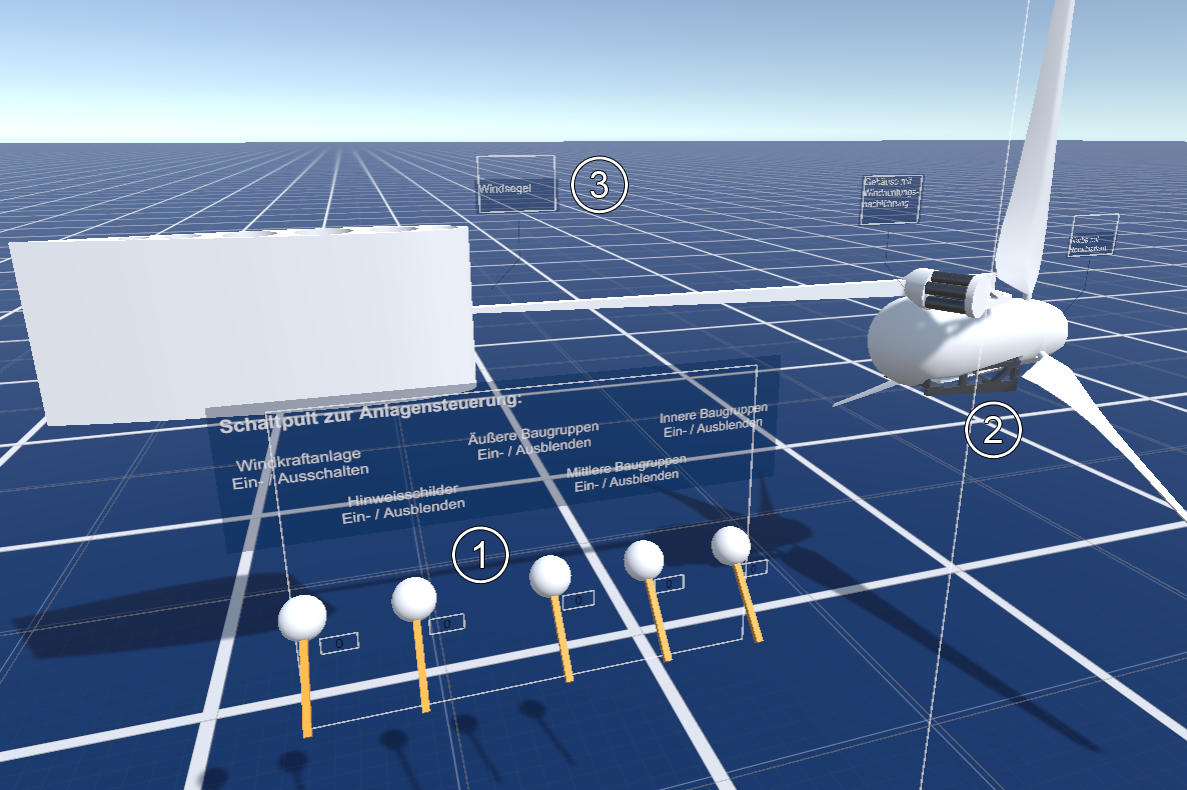
\includegraphics[keepaspectratio, width=1\textwidth]{bildquellen/szene}
	\caption{Szene in Unity.}
	\label{fig:4.1}
\end{figure}

Um die Szene zu strukturieren wurde die hierarchische Gruppierung vom VRTK-Framework übernommen. Diese der Szene untergeordneten GameObjects enthalten alle wichtigen Komponenten, welche für VR-Anwendung erforderlich sind. Die Folgende Struktur soll den hierarchischen Szenenaufbau verdeutlichen.

\begin{itemize}
\item[>] \textbf{Szene} 
	
	\begin{itemize}
	\item[>] \textbf{[VRTK\_SDKManager]:} Lädt Konfigurationen der SDKs (Windows MR, Oculus, SteamVR, UnityXR, VR-Simulator) und legt die Startreihenfolge fest.  	

		\begin{itemize}
			\item[>]\textbf{[VRTK\_SDKSetups]:} Enthält die Konfigurationsobjekte der oben genannten SDKs inklusive CameraRig, welches Kopf (Kamera) und Hände (Controller) beinhaltet.  		
		\end{itemize}
	
	\item[>] \textbf{[VRTK\_Scripts]}
	
	\item[>] \textbf{[SceneScripts]}
	
	\item[>] \textbf{SceneObjects}
	\end{itemize}
	
\end{itemize}

\section{Implementierte Usecases}
\label{sec:ImplementierteUsecases}
abc
